% Options for packages loaded elsewhere
% Options for packages loaded elsewhere
\PassOptionsToPackage{unicode}{hyperref}
\PassOptionsToPackage{hyphens}{url}
\PassOptionsToPackage{dvipsnames,svgnames,x11names}{xcolor}
%
\documentclass[
  portuguese,
]{estat/estat}
\usepackage{xcolor}
\usepackage[left=3cm,right=2cm,top=3cm,bottom=2cm]{geometry}
\usepackage{amsmath,amssymb}
\setcounter{secnumdepth}{5}
\usepackage{iftex}
\ifPDFTeX
  \usepackage[T1]{fontenc}
  \usepackage[utf8]{inputenc}
  \usepackage{textcomp} % provide euro and other symbols
\else % if luatex or xetex
  \usepackage{unicode-math} % this also loads fontspec
  \defaultfontfeatures{Scale=MatchLowercase}
  \defaultfontfeatures[\rmfamily]{Ligatures=TeX,Scale=1}
\fi
\usepackage{lmodern}
\ifPDFTeX\else
  % xetex/luatex font selection
  \setmainfont[]{Arial}
\fi
% Use upquote if available, for straight quotes in verbatim environments
\IfFileExists{upquote.sty}{\usepackage{upquote}}{}
\IfFileExists{microtype.sty}{% use microtype if available
  \usepackage[]{microtype}
  \UseMicrotypeSet[protrusion]{basicmath} % disable protrusion for tt fonts
}{}
\makeatletter
\@ifundefined{KOMAClassName}{% if non-KOMA class
  \IfFileExists{parskip.sty}{%
    \usepackage{parskip}
  }{% else
    \setlength{\parindent}{0pt}
    \setlength{\parskip}{6pt plus 2pt minus 1pt}}
}{% if KOMA class
  \KOMAoptions{parskip=half}}
\makeatother
% Make \paragraph and \subparagraph free-standing
\makeatletter
\ifx\paragraph\undefined\else
  \let\oldparagraph\paragraph
  \renewcommand{\paragraph}{
    \@ifstar
      \xxxParagraphStar
      \xxxParagraphNoStar
  }
  \newcommand{\xxxParagraphStar}[1]{\oldparagraph*{#1}\mbox{}}
  \newcommand{\xxxParagraphNoStar}[1]{\oldparagraph{#1}\mbox{}}
\fi
\ifx\subparagraph\undefined\else
  \let\oldsubparagraph\subparagraph
  \renewcommand{\subparagraph}{
    \@ifstar
      \xxxSubParagraphStar
      \xxxSubParagraphNoStar
  }
  \newcommand{\xxxSubParagraphStar}[1]{\oldsubparagraph*{#1}\mbox{}}
  \newcommand{\xxxSubParagraphNoStar}[1]{\oldsubparagraph{#1}\mbox{}}
\fi
\makeatother


\usepackage{longtable,booktabs,array}
\usepackage{calc} % for calculating minipage widths
% Correct order of tables after \paragraph or \subparagraph
\usepackage{etoolbox}
\makeatletter
\patchcmd\longtable{\par}{\if@noskipsec\mbox{}\fi\par}{}{}
\makeatother
% Allow footnotes in longtable head/foot
\IfFileExists{footnotehyper.sty}{\usepackage{footnotehyper}}{\usepackage{footnote}}
\makesavenoteenv{longtable}
\usepackage{graphicx}
\makeatletter
\newsavebox\pandoc@box
\newcommand*\pandocbounded[1]{% scales image to fit in text height/width
  \sbox\pandoc@box{#1}%
  \Gscale@div\@tempa{\textheight}{\dimexpr\ht\pandoc@box+\dp\pandoc@box\relax}%
  \Gscale@div\@tempb{\linewidth}{\wd\pandoc@box}%
  \ifdim\@tempb\p@<\@tempa\p@\let\@tempa\@tempb\fi% select the smaller of both
  \ifdim\@tempa\p@<\p@\scalebox{\@tempa}{\usebox\pandoc@box}%
  \else\usebox{\pandoc@box}%
  \fi%
}
% Set default figure placement to htbp
\def\fps@figure{htbp}
\makeatother



\ifLuaTeX
\usepackage[bidi=basic]{babel}
\else
\usepackage[bidi=default]{babel}
\fi
\ifPDFTeX
\else
\babelfont{rm}[]{Arial}
\fi
% get rid of language-specific shorthands (see #6817):
\let\LanguageShortHands\languageshorthands
\def\languageshorthands#1{}


\setlength{\emergencystretch}{3em} % prevent overfull lines

\providecommand{\tightlist}{%
  \setlength{\itemsep}{0pt}\setlength{\parskip}{0pt}}



 


\authors{%
    Estatiano 1 \\
    Estatiano 2\\
    Estatiano 3\\
}

% escreva o nome do cliente aqui
% se for mais de um separe por \\
\client{%
    ESTAT
}
% Baixando pacotes
\RequirePackage{fancyhdr}
\RequirePackage{graphicx}

\setlength\headheight{28pt}  

\setlength{\parindent}{15pt} % Adiciona indentação nos parágrafos
\setlength{\parskip}{0pt} % Adiciona 0 espaço entro os parágrafos

\let\oldsection\section
\renewcommand\section{\clearpage\oldsection}
\makeatletter
\@ifpackageloaded{float}{}{\usepackage{float}}
\floatstyle{plain}
\@ifundefined{c@chapter}{\newfloat{quadro}{h}{loquad}}{\newfloat{quadro}{h}{loquad}[chapter]}
\floatname{quadro}{Quadro}
\floatstyle{plaintop}
\restylefloat{quadro}
\newcommand*\listofquadros{\listof{quadro}{List of Testes}}
\makeatother
\makeatletter
\@ifpackageloaded{caption}{}{\usepackage{caption}}
\AtBeginDocument{%
\ifdefined\contentsname
  \renewcommand*\contentsname{Índice}
\else
  \newcommand\contentsname{Índice}
\fi
\ifdefined\listfigurename
  \renewcommand*\listfigurename{Lista de Figuras}
\else
  \newcommand\listfigurename{Lista de Figuras}
\fi
\ifdefined\listtablename
  \renewcommand*\listtablename{Lista de Tabelas}
\else
  \newcommand\listtablename{Lista de Tabelas}
\fi
\ifdefined\figurename
  \renewcommand*\figurename{Figura}
\else
  \newcommand\figurename{Figura}
\fi
\ifdefined\tablename
  \renewcommand*\tablename{Tabela}
\else
  \newcommand\tablename{Tabela}
\fi
}
\@ifpackageloaded{float}{}{\usepackage{float}}
\floatstyle{ruled}
\@ifundefined{c@chapter}{\newfloat{codelisting}{h}{lop}}{\newfloat{codelisting}{h}{lop}[chapter]}
\floatname{codelisting}{Listagem}
\newcommand*\listoflistings{\listof{codelisting}{Lista de Listagens}}
\captionsetup{labelsep=colon}
\makeatother
\makeatletter
\makeatother
\makeatletter
\@ifpackageloaded{caption}{}{\usepackage{caption}}
\@ifpackageloaded{subcaption}{}{\usepackage{subcaption}}
\makeatother
\usepackage{bookmark}
\IfFileExists{xurl.sty}{\usepackage{xurl}}{} % add URL line breaks if available
\urlstyle{same}
\hypersetup{
  pdflang={pt},
  colorlinks=true,
  linkcolor={black},
  filecolor={black},
  citecolor={black},
  urlcolor={black},
  pdfcreator={LaTeX via pandoc}}


\author{}
\date{}
\begin{document}

% Limpando tudo
\fancyhf{} 

% Ajustes do header
\fancyhead[L]{} % limpando o lado esquerdo
\fancyhead[R]{
\includegraphics[width=0.20\textwidth]{estat/imagens/estat.png}} % adicionando logo no canto direito
\renewcommand{\headrulewidth}{0pt}   % sem linha embaixo da logo

% Ajustes de fim de página
\fancyfoot[R]{\textcolor{white}{\thepage}} % Número em branco no canto direito

% Aplicando o estilo que acabamos de criar
\pagestyle{fancy} 


\labelformat{quadro}{\textbf{#1}}

\renewcommand*\contentsname{Sumário}
{
\hypersetup{linkcolor=}
\setcounter{tocdepth}{3}
\tableofcontents
}

\begin{verbatim}
\begin{quadro}[H]
    \setlength{ \tabcolsep}{9pt}
    \renewcommand{  \arraystretch}{1.20}
    \caption{Medidas resumo da(o) [nome da variável]}
    \centering
    \begin{adjustbox}{max width=\textwidth}
    \begin{tabular} { | l |
            S[table-format = 1.2]
            |}
    \hline
        \textbf{Estatística} & \textbf{Valor} \\
        \hline
        Média & 11,79 \\
        Desvio Padrão & 5,12 \\
        Variância & 26,23 \\
        Mínimo & 2 \\
        1º Quartil & 8,44 \\
        Mediana & 11,25 \\
        3º Quartil & 14,25 \\
        Máximo & 26,5 \\
    \hline
    \end{tabular}
    \label{quad:quadro_resumo1}
    \end{adjustbox}
\end{quadro}
\begin{quadro}[H]
    \setlength{ \tabcolsep}{9pt}
    \renewcommand{  \arraystretch}{1.20}
    \caption{Medidas resumo da(o) [nome da variável]}
    \centering
    \begin{adjustbox}{max width=\textwidth}
    \begin{tabular} { | l |
            S[table-format = 1.2]
            |}
    \hline
        \textbf{Estatística} & \textbf{Valor} \\
        \hline
        Média & 5,01 \\
        Desvio Padrão & 3,76 \\
        Variância & 14,12 \\
        Mínimo & -4,44 \\
        1º Quartil & 2,92 \\
        Mediana & 4,5 \\
        3º Quartil & 7,5 \\
        Máximo & 12,95 \\
    \hline
    \end{tabular}
    \label{quad:quadro_resumo1}
    \end{adjustbox}
\end{quadro}
\end{verbatim}

\section{Análises}\label{anuxe1lises}

\subsection{Relação entre SELIC e juros
reais}\label{relauxe7uxe3o-entre-selic-e-juros-reais}

Esta análise tem como objetivo investigar a relação linear entre a taxa
Selic e os juros reais no período de 2002 a 2022.

Para a realização da análise, foram consideradas duas variáveis
quantitativas contínuas:

selic\_meta: corresponde à taxa Selic, a taxa básica de juros da
economia;

juros\_reais: representa a taxa de juros real, ou seja, a taxa nominal
descontada da inflação.

Na análise estatística descritiva, foram calculadas medidas de tendência
central, dispersão e posição para ambas as variáveis.

\begin{quadro}[H]

\caption{\label{quad-quadro_selic}Medidas de resumo da taxa selic}

\centering{

    \begin{tabular} { | l |
            S[table-format = 1.2]
            |}
    \hline
        \textbf{Estatística} & \textbf{Valor} \\
        \hline
        Média & 14,35 \\
        Desvio Padrão & 4,75 \\
        Variância & 22,55 \\
        Mínimo & 7,25 \\
        1º Quartil & 10,94 \\
        Mediana & 13 \\
        3º Quartil & 18 \\
        Máximo & 26,5 \\
    \hline
    \end{tabular}

}

\end{quadro}%

\begin{quadro}[H]

\caption{\label{quad-quadro_juros}Medidas de resumo dos juros reais}

\centering{

    \begin{tabular} { | l |
            S[table-format = 1.2]
            |}
    \hline
        \textbf{Estatística} & \textbf{Valor} \\
        \hline
        Média & 5,01 \\
        Desvio Padrão & 3,76 \\
        Variância & 14,12 \\
        Mínimo & -4,44 \\
        1º Quartil & 2,92 \\
        Mediana & 4,5 \\
        3º Quartil & 7,5 \\
        Máximo & 12,95 \\
    \hline
    \end{tabular}

}

\end{quadro}%

A partir do \textbf{Quadro}~\ref{quad-quadro_selic} e
\textbf{Quadro}~\ref{quad-quadro_juros}, percebe-se a proximidade entre
a média e a mediana das duas variáveis, apesar de ambas apresentarem
valores extremos que indicam certa dispersão nos dados. No caso da taxa
Selic, observa-se um valor máximo consideravelmente alto em comparação à
média; já para os juros reais, nota-se, a partir do valor mínimo, a
ocorrência de juros reais negativos.

Com o intuito de observar a relação linear entre a taxa Selic e os juros
reais, construi-se um gráfico de dipersão - uma representação gráfica
utilizada para ilustrar o comportamento conjunto de duas variáveis
quantitativas, neste caso, selic\_meta e juros\_reais.

\begin{figure}[H]

\caption{\label{fig-selic-vs-juros}Gráfico de dispersão da taxa selic
pelos juros reais (2002-2012)}

\centering{

\pandocbounded{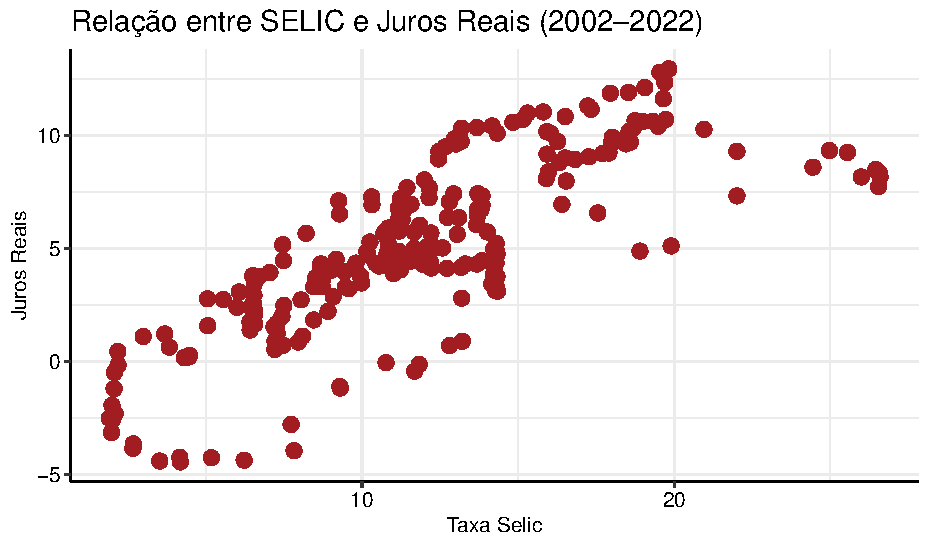
\includegraphics[keepaspectratio]{joaofabio_files/figure-pdf/fig-selic-vs-juros-1.pdf}}

}

\end{figure}%

Cada ponto na \(\ref{fig-selic-vs-juros}\), representa um par ordenado,
composto pela taxa Selic e os juros reais em determinado mês, permitindo
visualizar padrões, correlações e possíveis tendências.

Como pode ser observado na \(\ref{fig-selic-vs-juros}\), o gráfico de
dispersão apresenta uma relação positiva entre as variáveis. Percebe-se
que, à medida que a taxa selic aumenta, os juros reais também tendem a
aumentar. Entretanto, nota-se que, a partir do momento em que a taxa
Selic atinge aproximadamente 20\%, os juros reais deixam de crescer
proporcionalmente, o que pode estar relacionado com um aumento
significativo da inflação.

Para compreender a natureza e força dessa relação, foi realizada uma
regressão linear simples. Uma regressão linear é uma técnica estatística
usada para estimar a relação entre variáveis.

\begin{figure}[H]

\caption{\label{fig-selic-vs-juros-regressao-lin}Gráfico de dispersão da
taxa selic pelos juros reais (2002-2012)}

\centering{

\pandocbounded{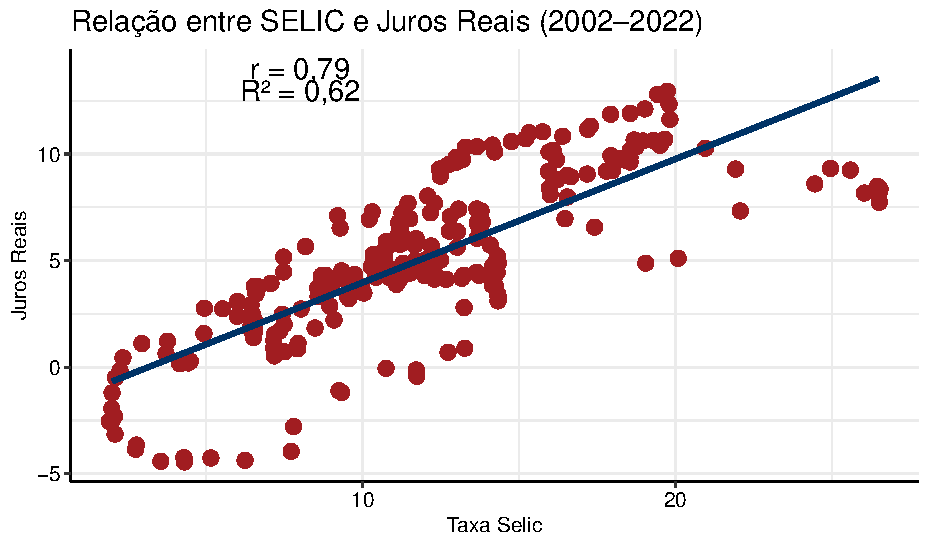
\includegraphics[keepaspectratio]{joaofabio_files/figure-pdf/fig-selic-vs-juros-regressao-lin-1.pdf}}

}

\end{figure}%

A análise de regressão linear mostra uma relação linear positiva entre a
taxa Selic e os juros reais. O coeficiente da taxa Selic calculado em
0,579 revela que os juros simples aumentam aproximadamente 0,58 pontos
percentuais a cada 1 ponto percentual na taxa Selic.

Ao estimar o coeficiente de correlação de Pearson - medida que verifica
o grau de relação linear entre duas variáveis quantitativas,
representada pela letra r -, o valor encontrado foi de aproximadamente
0,79. Isso indica uma correlação linear positiva forte, ou seja, existe
uma relação positiva entre as variáveis selic\_meta e juros\_reais, como
se fossem diretamente proporcionais. Entretanto, o coeficiente de
Pearson indica uma tendência e não é uma garantia de proporcionalidade.
Isso é evidenciado na \(\ref{fig-selic-vs-juros-regressao-lin}\), onde
se observa que, em determinados pontos em que a taxa Selic está em torno
de 20\%, os juros reais são menores do que em outros pontos em que a
Selic está por volta de 10\%.

O coeficiente de determinação (R²) também foi estimado, já que explica a
variância global dos dados. O valor encontrado de aproximadamente 0,62,
sugere que 62\% da variação dos juros reais pode ser explicada pela taxa
Selic.

A partir da análise realizada, consegue-se inferir que a taxa Selic tem
uma forte influência sobre o comportamento dos juros reais. Entretanto,
como os juros reais são obtidos pela taxa nominal descontada da
inflação, fica evidente que a Selic, isoladamente, não é capaz de
explicar completamente a variação dos juros reais.




\end{document}
